%
% File: chap01.tex
% Author: Joshua Carey

%
\let\textcircled=\pgftextcircled
\chapter{Background}\label{chap:background}

% \initial{T}his chapter delves into the application of machine learning in sailboat control, with a particular emphasis on utilizing kites as a means of propulsion. The exploration of kite-powered vessel technologies presents a novel avenue to enhance the efficiency of sailboats. The fusion of machine learning, specifically Reinforcement Learning (RL), with kite propulsion systems, opens up a realm of possibilities for autonomous sailboat control. 



% The subsequent sections will provide an in-depth examination of kite-powered vessel technologies, introduce the core concepts of RL, discuss relevant literature, identify gaps in current research, and highlight the novelty and potential contributions of the proposed work. 

\initial{T}he maritime domain has long been a focal point of innovation and technological advancement. Historically, propulsion mechanisms have evolved from rudimentary oars to sophisticated sails, each iteration seeking to harness nature's forces more efficiently. Today, as we stand at the intersection of technology and tradition, there emerges a compelling avenue for exploration: kite-powered vessels. This innovative approach to propulsion seeks to leverage the aerodynamic advantages of kites, offering potential enhancements in efficiency and maneuverability over traditional sails.

However, the introduction of kites as a propulsion mechanism brings forth a new set of challenges. The dynamic nature of kites, combined with the unpredictable marine environment, necessitates advanced control systems capable of real-time adaptation and decision-making. This is where the application of machine learning, and more specifically Reinforcement Learning (RL), becomes paramount. An RL agent learns to make decisions that maximize a certain objective, often framed as a cumulative reward. The potential of RL in maritime propulsion is evident: it offers a framework for developing control systems that can adapt to changing conditions and environments.

REPHRASE THE NEXT BIT
\newline
This chapter aims to provide a comprehensive overview of the current state of kite-powered vessel technologies, with a particular emphasis on the integration of RL-based control systems. Through a detailed examination of relevant literature, we will identify existing research gaps, underscore the significance of the proposed work, and set the stage for the subsequent sections.

As we navigate through this background, we will delve into the core concepts of RL and discuss the algorithms behind it. We will also look at its relevance to maritime propulsion, and its potential in revolutionizing the way we think about sailing.

\section{Reinforcement Learning (RL)}\label{RL_background}
% User
% Write me a technical and informative introduction for Reinforcement Learning (RL). This is part of the background section of a thesis and will lay the foundation for how and why RL can/has/might want to be used to control boats (and kites instead of sails). Make it about 1000 words and include citations for your sources. The style should be informative but upbeat. 

Reinforcement Learning (RL) is a paradigm of machine learning that has been making waves, both literally and figuratively, in the vast sea of artificial intelligence (AI). At its core, RL is about learning by interaction: an agent takes actions in an environment to maximize some notion of cumulative reward. The agent learns from the consequences of its actions, rather than from being explicitly taught, making it a powerful tool for tasks where the optimal strategy is unknown or hard to define$~$\cite{sutton2018reinforcement}.

Imagine teaching a child to ride a bicycle. You don't provide a step-by-step manual; instead, the child learns by trying different actions (like pedaling or balancing) and receiving feedback (falling down or moving forward). This trial-and-error approach is the essence of RL. The agent (in this case, the child) interacts with its environment (the bicycle and the ground) and learns a policy that dictates the best action to take in any given situation based on the rewards (or penalties) it receives$~$\cite{watkins1992qlearning}. Figure$~$\ref{fig:rl_diagram} illustrates this process.

\begin{figure}
    \centering
    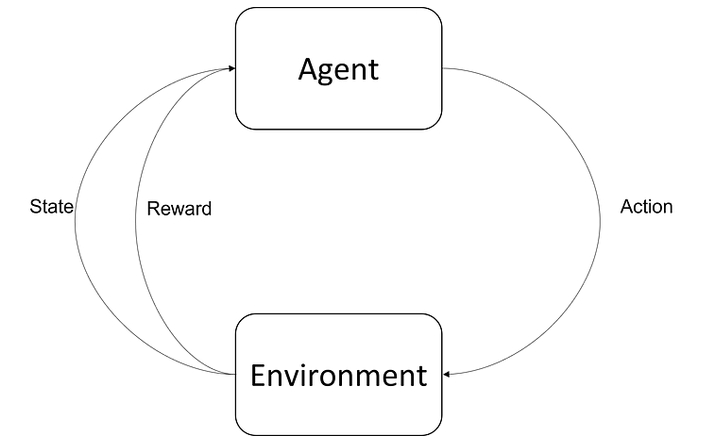
\includegraphics[width=0.8\textwidth]{Images/RL_Loop.png}
    \caption{A diagram of the RL Loop}
    \label{fig:rl_diagram}
\end{figure}

Historically, RL has its roots in the fields of operations research and behavioral psychology. The idea of learning optimal strategies through interaction has been explored in various contexts, from game playing to industrial optimization$~$\cite{bellman1957dynamic}. However, it's the recent advancements in computational power and algorithms that have propelled RL to the forefront of AI research. Games like Go, which were once considered too complex for computers to master, have now been conquered by RL agents, showcasing the immense potential of this approach\cite{silver2016mastering}.

Now, to explore how RL can be applied to the maritime world. Boats, with their intricate dynamics and the unpredictable nature of water, present a challenging environment for control systems. Traditional control methods often rely on predefined rules and heuristics, which might not always be optimal, especially in changing conditions. These autonomous controls vary from something as simple as a piece of bungee to PID controllers to more complex systems like Model Predictive Control (MPC). Enter RL. With its ability to learn from experience, an RL-based control system can adapt to varying conditions, ensuring smooth sailing even in turbulent waters, gusty winds$~$\cite{yang2020reinforcement}.

But why stop at boats? The concept of using kites to harness wind power for propulsion is not new. Historically, kites have been used in various cultures for fishing, transportation, and even warfare$~$\cite{hallion2003taking}. In the modern context, kites offer an exciting alternative to traditional sails, providing more power and maneuverability. However, controlling a kite, especially in varying wind conditions, is a complex task.  Kite control has only been explored in recent years, primarily in the field of renewable energy, where large ram-air kites are used to harness wind power for electricity generation$~$\cite{kitecontrol}. However these problems are static and do not handle situations where the base of the kite is moving. This is where RL shines. By continuously interacting with the environment and adjusting the kite's position and angle, an RL agent can learn the optimal control strategy to harness the maximum wind power, propelling the boat efficiently$~$\cite{erhard2013control}.

The potential applications of RL in marine navigation are vast. From optimizing routes for cargo ships to ensuring safe navigation in crowded ports, the possibilities are as vast as the open sea. Moreover, as environmental concerns become more pressing, the need for efficient and sustainable maritime solutions becomes paramount. RL, with its ability to optimize and adapt, can play a pivotal role in addressing these challenges$~$\cite{christiansen2013ship}.

In conclusion, Reinforcement Learning is not just another tool in the AI toolkit; it's a paradigm shift in how we approach problem-solving. Its potential in the maritime world is just beginning to be tapped. As we venture into the future, with boats steered by intelligent agents and sails replaced by kites controlled with precision, it's clear that RL will be at the helm, guiding us towards uncharted territories and new horizons\cite{mnih2015humanlevel}.

\section{Unity Game Engine}

Unity, a name that resonates with game developers and enthusiasts alike, stands as a beacon in the realm of game development. Born in the vibrant city of Copenhagen, Denmark, in 2005, Unity has since evolved into a powerhouse, democratizing game development and breathing life into iconic games like `Among Us' and `Pokemon Go' \cite{unity100seconds}.

At its heart, Unity is a cross-platform game engine designed to craft both 2D and 3D experiences. It offers a harmonious blend of a powerful graphical editor and the flexibility of \texttt{C\#} coding, allowing developers to translate their visions into virtual realities \cite{unitymanual2021}. While the engine's core is written in C++, it graciously opens its arms to developers familiar with \texttt{C\#}, making the development process both intuitive and efficient.

Diving into the basics of Unity game development, one is greeted with a plethora of tools and components that simulate real-world interactions. Unity's lighting, physics, rigidbody, and colliders work in tandem to create immersive environments. Whether it's the glint of sunlight reflecting off a surface or the realistic bounce of a ball, Unity ensures every detail is just right \cite{goldstone2010}. Developers can further enhance objects with custom \texttt{C\#} scripts, paving the way for unique gameplay experiences.

Imagine crafting a game level: a dodgeball arena illuminated by a radiant light source, with a camera capturing every thrilling moment. Unity makes this possible with simple objects like planes, cylinders, and spheres. The intuitive interface allows developers to select, move, rotate, and scale objects with ease, setting the stage for an exhilarating match \cite{harrison2013}.

But what's a game without some action? Unity's rigid body component breathes life into objects, allowing them to be influenced by gravity. Combine this with the material component, and you can create mesmerizing visual effects, from the sheen of a metallic surface to the rough texture of a stone \cite{blackman2012}.

Unity's commitment to realism and smooth gameplay is further evident in its two types of updates: Update and FixedUpdate. While the former is called every frame during gameplay, ensuring fluid animations and interactions, the latter syncs with the physics engine's frame rate, making it ideal for moving objects around \cite{unityupdatefixedupdate}.

Now, envision a player navigating this dodgeball arena, deftly maneuvering with the arrow keys, while a ball rolls with momentum as the game begins. Unity makes this possible with simple input methods in the FixedUpdate and scripts that add force to objects \cite{unityrigidbody}.

Unity's ML-Agents toolkit is a game-changer for those looking to infuse artificial intelligence into their games. ML-Agents provides a platform to train intelligent agents within the Unity environment using Reinforcement Learning, imitation learning, and more. This makes it an ideal choice for complex simulations like kiteboat training, where agents can learn optimal strategies through interaction.

In conclusion, Unity is not just a game engine; it's a canvas for creativity, a platform for innovation, and a testament to the limitless possibilities of virtual worlds. As we set sail in our virtual kiteboat, with the winds of Unity propelling us forward, the horizon looks promising and full of potential.

\section{Proximal Policy Optimization (PPO)}\label{sec:ppo_background}

Reinforcement Learning (RL) has witnessed a plethora of algorithms, each striving to optimize policy in its unique way. Among these, the Proximal Policy Optimization (PPO) algorithm stands out as a beacon of efficiency and simplicity \cite{schulman2017ppo}.

PPO is a member of the policy gradient family of RL algorithms. Unlike traditional policy gradient methods that perform a single gradient update per data sample, PPO introduces a "surrogate" objective function. This novel approach allows for multiple epochs of minibatch updates, optimizing the policy over a series of iterations. The essence of PPO lies in its ability to alternate between sampling data through interaction with the environment and optimizing the surrogate objective using stochastic gradient ascent.

The inception of PPO was driven by the need for an algorithm that combined the best of all worlds: scalability, data efficiency, and robustness. While deep Q-learning and vanilla policy gradient methods have their merits, they often fall short in terms of data efficiency and robustness. Trust Region Policy Optimization (TRPO), on the other hand, although effective, is relatively intricate and lacks compatibility with certain architectures \cite{engstrom2020implementation}.

PPO seeks to bridge these gaps. It aims to achieve the data efficiency and consistent performance of TRPO but does so using only first-order optimization. The brilliance of PPO is encapsulated in its objective with clipped probability ratios. This objective provides a pessimistic estimate (or a lower bound) of the policy's performance. The optimization process in PPO is iterative, alternating between data sampling from the policy and performing several epochs of optimization on this sampled data.

Empirical evidence underscores the efficacy of PPO. When pitted against various versions of the surrogate objective, PPO, with its clipped probability ratios, emerges as the top performer. Furthermore, in head-to-head comparisons with other algorithms, PPO shines brightly. On continuous control tasks, PPO outperforms its competitors. In the realm of Atari games, PPO showcases superior sample complexity compared to A2C and performs on par with ACER, all while maintaining a simpler architecture.

The key characteristic of PPO is that it is an on-policy algorithm, meaning that it learns from the most recent experiences and that it uses an `actor-critic' method. The actor-critic method is a combination of two neural networks, the actor and the critic. The actor is responsible for learning the optimal policy, while the critic is responsible for evaluating the actions of the actor by estimating the value function.  

The actor-critic method can be broken down into the following steps:
\begin{enumerate}
    \item \textbf{Actor}: The actor network proposes an action given in the current state. The action is drawn from a probability distribution (the policy $\pi$) parameterized by the networks weights.
    \item \textbf{Critic}: The critic network estimates the value function $V(s)$ $V(s)$, which predicts the expected return (sum of future rewards) from state s under the current policy.
    \item \textbf{Advantage Estimation}: The advantage function $A(s,a)$ quantifies how much better taking a particular action aa is, compared to the average action in state ss, and is computed as 
    \begin{equation}
        A(s,a) = Q(s,a) - V(s)
    \end{equation}
    where $Q(s,a)$ is the action-value function, which is the expected return after taking action a in state s.
    \item \textbf{Objective Function}:  PPO optimizes a clipped surrogate objective function to prevent large policy updates, which could lead to performance collapse. The objective function $L^{CLIP}$ is defined as
    \begin{equation}
        L^{CLIP}(\theta) = \hat{\mathbb{E}}_t[min(r_t(\theta)\hat{A}_t, clip(r_t(\theta), 1-\epsilon, 1+\epsilon)\hat{A}_t)]
    \end{equation}
    were $r_t(\theta)$ is the probability ratio between the new and old policy, $\hat{A}_t$ is the advantage at time step $t$, and $\epsilon$ is a hyperparameter that controls the size of the policy update.
    \item \textbf{Policy Update}: PPO uses this objective to update the actor network's weights, maximizing the expected return while avoiding too large policy updates.
    \item textbf{Value Function Loss}: The critic network is trained to minimize the value function loss, which is typically the Mean Squared Error between the estimated value function V(s) and the observed return R.
    \item textbf{Entropy Bonus}: To encourage exploration, PPO adds an entropy bonus to the objective function, which promotes diversity in the action distribution.
\end{enumerate}

PPO iterates between sampling data through interaction with the environment and optimizing the clipped objective function using stochastic gradient ascent. This optimization is typically done using minibatch updates for efficiency.

By employing PPO, the agent learns to balance exploration (trying new actions) with exploitation (taking known rewarding actions), which is particularly effective for complex tasks like sailing a kiteboat where the agent must adapt to dynamic conditions and long-term consequences of actions.

\begin{figure}
    \centering
    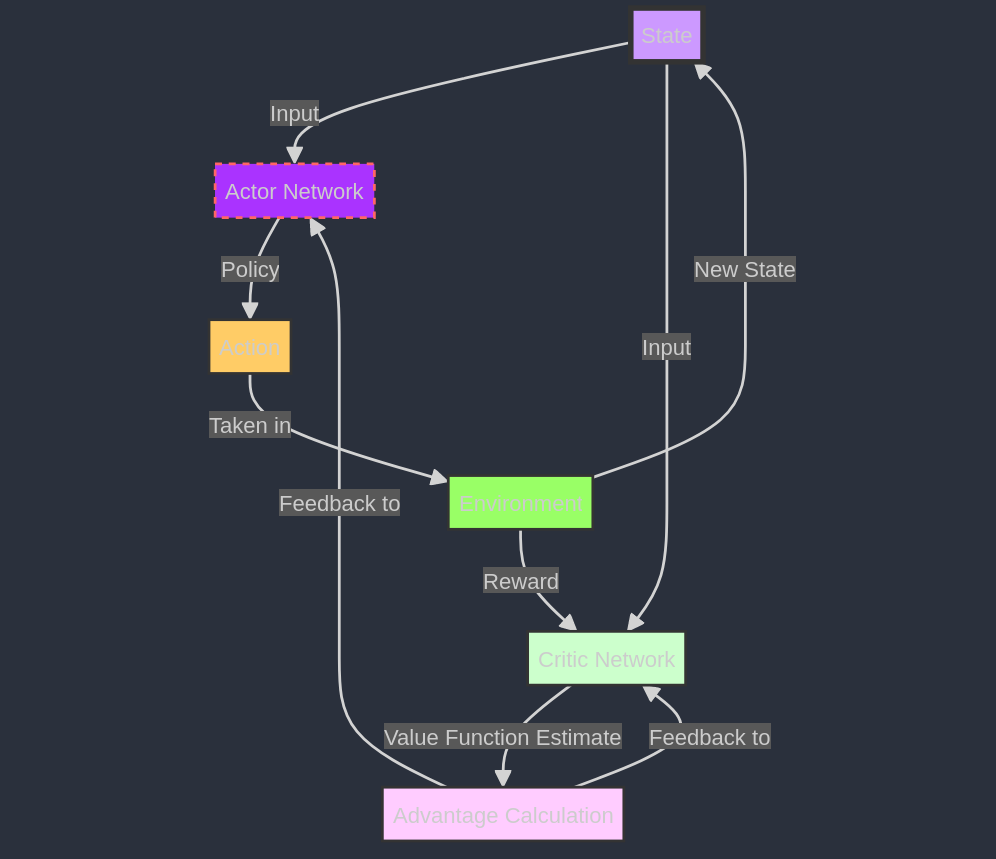
\includegraphics[width=0.5\textwidth]{Images/ppo_explanation.png}
    \caption{Actor-Critic Method}\label{actor_critic}
\end{figure}

But the story doesn't end with PPO alone. Unity's ML-Agents toolkit, which was touched upon earlier, seamlessly integrates with PPO. ML-Agents provides a platform for training intelligent agents within the Unity environment, and when combined with the power of PPO, it paves the way for robust and efficient training regimes. This synergy between PPO and ML-Agents is particularly promising for complex simulations, such as kiteboat training, where agents can iteratively learn and refine their strategies for optimal performance.

The Proximal Policy Optimization algorithm is a testament to the continuous evolution and innovation in the field of Reinforcement Learning. Its simplicity, efficiency, and robustness make it a prime choice for a myriad of applications. As we harness the combined power of PPO with Unity's ML-Agents for kiteboat simulations.



